\documentclass{article}
\usepackage[utf8]{inputenc}
\usepackage{graphicx}
\usepackage{booktabs} % For professional tables
\usepackage{amsmath}  % For math symbols like delta
\usepackage{float}    % For [H] placement
\usepackage{geometry}
\usepackage[hidelinks]{hyperref} % hidelinks removes colored boxes around links
\usepackage[justification=centering]{caption} % Center-align figure captions
\geometry{a4paper, margin=1in}

% Natbib for APA style citations (Author, Year)
\usepackage{cite}

\title{AI-Enabled Vision-Based Proximity Monitoring for Construction Safety             }
\author{}
\date{January 2026}

\begin{document}

\maketitle

\begin{abstract}
This study demonstrates how AI-enabled vision systems can enhance construction safety practice when designed and deployed with explicit attention to practical site conditions, system assumptions, and human-centered decision-making. We present a real-time, vision-based proximity monitoring system that integrates monocular depth estimation (RT-MonoDepth) and object detection (YOLOv11) within a unified pipeline, using only a single RGB camera. A key technical contribution is an automatic scale calibration approach that uses detected personnel as anthropometric reference objects, enabling approximate metric distance estimation without requiring stereo cameras, LiDAR, or manual calibration procedures. The system executes depth estimation, object detection, spatial reconstruction, and proximity analysis concurrently in a multi-stage, parallelized perception pipeline. To strengthen external validity, we additionally introduce an \emph{LLM-supervisor validation} protocol in which a locally hosted large language model (Llama~3.1 8B served via Ollama) is queried with thirty automatically graded questions whose ground truth is derived from the perception pipeline's structured CSV logs. Experimental evaluation on the KITTI benchmark demonstrates 96.09\% depth accuracy ($\delta < 1.25$), while the object detection model achieves 84.99\% mAP@50 on construction safety classes. Deployment assessment shows the integrated system achieves 22--25 FPS on consumer-grade processors and 11 FPS on a 2019 NVIDIA Jetson Nano after optimization. The LLM-supervisor evaluation reveals a clear capability gradient: 80\% accuracy on row-level lookups but 0\% on threshold-based proximity reasoning, providing direct empirical evidence that the deterministic CSV logger---rather than an LLM---must remain the system of record for safety-critical aggregation. The findings demonstrate that AI-enabled vision systems can transform ordinary video feeds into actionable safety intelligence while highlighting operational constraints---including camera placement, lighting conditions, occlusions, embedded model assumptions, and the limits of natural-language supervisors---that shape system performance in practice. This work contributes to a grounded understanding of AI as a socio-technical component of construction safety systems, emphasizing its role as a decision-support tool that augments rather than replaces professional judgment.
\end{abstract}

\textbf{Keywords:} AI-Enabled Safety Monitoring, Monocular Depth Estimation, Computer Vision, Construction Safety, YOLOv11, Real-Time Systems, Proximity Detection, Decision Support Systems, Large Language Models, LLM-as-Supervisor.

\section{Introduction}
The construction industry is one of the most dangerous sectors worldwide, with "struck-by-equipment" incidents being a leading cause of fatalities \cite{pan2021}. To mitigate these risks, artificial intelligence and computer vision systems are increasingly being explored to provide proactive risk management and turn reactive safety protocols into preventative ones \cite{badhan2025, vasquez2025}. Comprehensive reviews of deep-learning deployments confirm that state-of-the-art computer vision now possesses the robustness necessary to transition from academic prototypes to continuously operational site-surveillance tools \cite{cai2025}. Two key technologies have emerged as foundational for this goal: object detection and depth estimation. Advances in object detection, particularly with models like YOLO, have enabled robust, real-time identification and segmentation of critical agents like workers and machinery on complex construction sites, including PPE enforcement in occluded environments \cite{he2024, zhang2024helmets, ge2025, pan2021}. Concurrently, monocular depth estimation (MDE) has matured into a cost-effective alternative to expensive hardware like LiDAR, with modern lightweight networks achieving real-time performance on embedded systems \cite{feng2024, masoumian2022, cheng2025, ma2026}. Cross-domain insights from autonomous driving research further enrich this landscape, providing proven depth estimation algorithms directly applicable to preventing struck-by incidents on active sites \cite{huang2025}. These models can generate dense depth maps from a single, inexpensive camera, providing crucial spatial information about a scene.

Despite these parallel advancements, a critical gap remains between the capabilities of individual models and the needs of a practical, deployable safety system. Object detection answers what an object is but provides no spatial depth. MDE, conversely, provides spatial data but lacks semantic understanding and is fundamentally limited by an inherent scale ambiguity—its output is a relative depth map without real-world units, rendering it unusable for metric distance measurement \cite{zhang2025, shen2023}. This ambiguity has been a primary barrier preventing the widespread adoption of MDE for safety-critical applications.

While the potential of fusing these two technologies has been explored, for example in the YOLO MDE framework \cite{yu2021}, the challenge of resolving scale ambiguity in a practical, on-the-fly manner persists. Many approaches still fall short of providing a truly deployable solution that can operate with uncalibrated, monocular cameras in dynamic environments. This paper bridges this gap by introducing a unified framework that synergistically integrates state-of-the-art object detection (YOLOv11) and MDE (RT-MonoDepth) into a single, end-to-end system. Our primary contribution is a novel automatic geometric calibration method that resolves scale ambiguity by using detected personnel as an anthropometric reference, enabling the system to produce precise, object-specific distance measurements in meters from a single uncalibrated camera. By running these models concurrently in a multi-threaded pipeline, our system transforms standard 2D video into an actionable source of 3D spatial intelligence, creating a deployable safety tool that can proactively identify and log proximity hazards in real-time on construction sites.

A second contribution---and a direct response to the validation requirements of safety-critical AI---is an \emph{LLM-as-supervisor} evaluation protocol. Rather than restricting validation to numerical accuracy on benchmarks, we treat the system's persistent CSV logs as the ground truth and use a locally hosted Llama~3.1 8B model \cite{dubey2024llama,ollama2024} to answer thirty automatically graded questions spanning detection counts, depth and confidence aggregates, row-level lookups, threshold-based proximity reasoning, and supervisory safety decisions. This protocol is motivated by recent work demonstrating both the promise and the limits of vision-language models for hazard identification \cite{adil2025}, RAG-grounded frameworks for automated safety inspection \cite{wang2025}, and comparative analyses of retrieval-augmented versus fine-tuned LLMs for construction knowledge queries \cite{lee2024}. Structured prompting strategies informed by AEC-domain prompt engineering research \cite{samsami2024} further shape the evaluation harness design. This protocol stress-tests an increasingly common deployment pattern in which a free-form natural-language assistant is layered on top of a deterministic perception pipeline, and it produces a quantitative, reproducible answer to the question of \emph{when an LLM may, and may not, be trusted to summarize safety telemetry}.

\section{Methods}

\subsection{System Architecture and Real-Time Processing Pipeline}
The methodology is built upon the RT-MonoDepth framework, a comprehensive real-time computational pipeline engineered specifically for construction site monitoring applications through the synergistic integration of monocular depth estimation and semantic object detection algorithms. The system architecture processes continuous video streams through a sophisticated multi-modal input acquisition pipeline, generating dense disparity maps augmented with object-specific semantic metadata and spatial relationships without requiring stereo-pair camera configurations or active depth sensing hardware.

\begin{figure}[H]
    \centering
    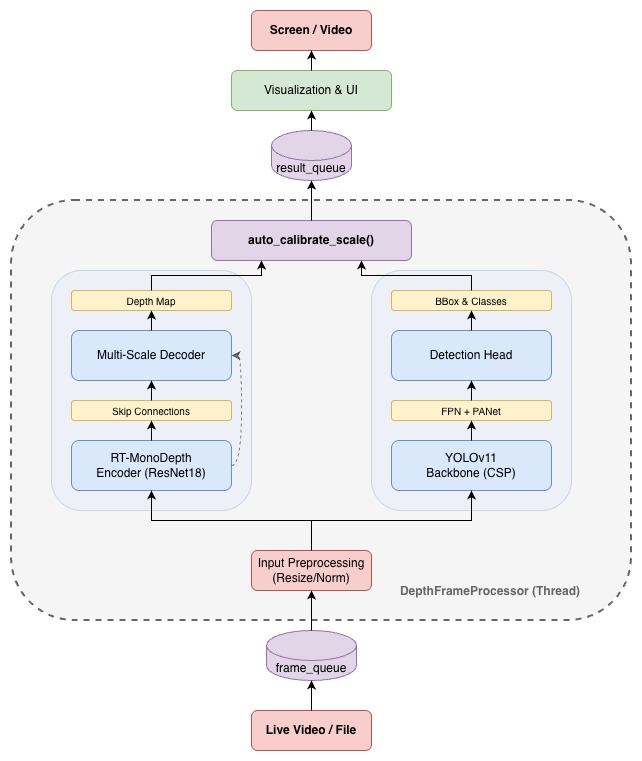
\includegraphics[width=0.65\linewidth]{figure1_architecture.jpg}
    \caption{The parallel processing architecture, demonstrating the concurrent execution paradigm that enables real-time performance characteristics. The system processes video frames through dual ML pipelines (RT-MonoDepth and YOLOv11) with queue-based synchronization.}
    \label{fig:architecture}
\end{figure}

The core architectural foundation employs the RT-MonoDepth neural network, utilizing a sophisticated ResNet encoder-decoder topology with skip connections to infer metric depth information from monocular RGB images \cite{feng2024}. The system integrates platform-specific hardware acceleration libraries, including MLX optimization for Apple Silicon architectures and CUDA acceleration for NVIDIA embedded platforms such as Jetson series processors, achieving sustained processing throughputs exceeding 30 FPS with end-to-end computational latency under 50ms.

\subsection{Multi-threaded Parallel Processing Architecture and Real-time Optimization}
The system's real-time performance characteristics are achieved through a sophisticated parallel processing architecture (Figure \ref{fig:architecture}), orchestrated by the \texttt{realtime\_depth\_video.py} script managing data ingestion from heterogeneous input modalities including live webcam feeds, pre-recorded video sequences, and real-time streaming protocols. The architecture implements a producer-consumer threading paradigm with minimalist queue-based buffering mechanisms designed to mitigate computational latency and ensure responsive real-time operation under varying processing loads. The threading architecture utilizes dual-queue synchronization primitives implemented through Python's \texttt{threading.Queue} interface: a primary \texttt{frame\_queue} and bidirectional \texttt{result\_queue}, each configured with maximum buffer capacity of unity (\texttt{maxsize=1}). This configuration implements an intelligent automatic frame-dropping mechanism that prevents accumulation of temporal artifacts in memory buffers while facilitating lock-free concurrent execution when processing pipeline latency exceeds frame acquisition intervals. The zero-copy memory management approach minimizes data transfer overhead between processing threads. A dedicated \texttt{DepthFrameProcessor} thread, implemented as a subclass of \texttt{threading.Thread}, orchestrates concurrent execution of the primary machine learning inference engines. This specialized thread manages simultaneous RT-MonoDepth depth estimation and YOLOv11 object detection inference operations on identical input frame tensors, enabling true parallel processing without blocking the main visualization and user interface loops. The parallelized architectural design isolates distinct computational tasks including frame acquisition, ML model inference, sensor fusion processing, and output rendering, thereby preventing blocking I/O operations while maintaining fluid user interface responsiveness and system stability.

\begin{figure}[H]
    \centering
    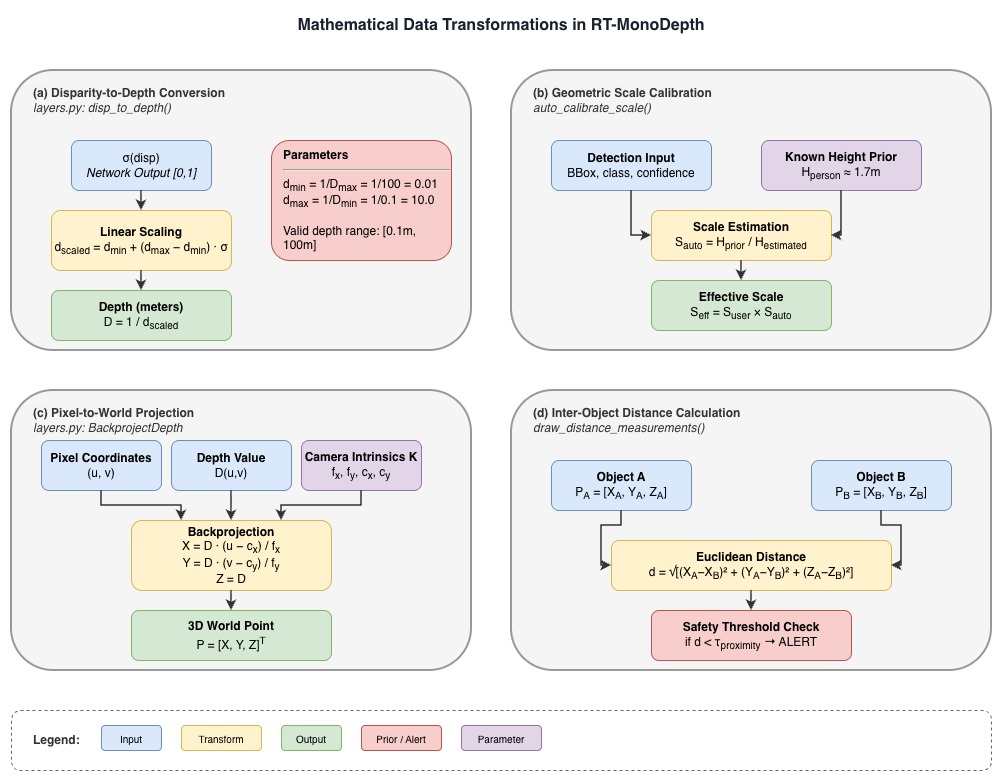
\includegraphics[width=0.85\linewidth]{figure2_data_transformation.jpg}
    \caption{Mathematical data transformation flow illustrating the sequential processing stages from raw RGB input through disparity estimation to final 3D world coordinate generation. The diagram details the disparity-to-depth conversion, geometric scale calibration, pixel-to-world projection, and inter-object distance calculation.}
    \label{fig:data_transformation}
\end{figure}

\subsection{Monocular Depth Estimation Neural Architecture and Implementation}
The depth estimation module implements RT-MonoDepth, a neural network architecture derived from the Monodepth2 framework with substantial architectural optimizations for high-throughput real-time inference applications \cite{feng2024}. The system incorporates dynamic model selection capabilities, automatically detecting and deploying either the full-scale DepthDecoder or computationally optimized compact DepthDecoderS model variants based on weight file path analysis and system resource availability. As illustrated in the data transformation flow (Figure \ref{fig:data_transformation}), the neural network processes raw RGB input tensors with standardized spatial dimensions of $640 \times 480 \times 3$ pixels through a comprehensive preprocessing pipeline including aspect ratio preservation, color space normalization, and tensor standardization. The architecture comprises two primary computational components integrated through residual connections. The encoder network utilizes hierarchical convolutional feature extraction layers implementing multi-scale spatial representation learning. The ResNet backbone architecture captures contextual semantic information through progressively deeper feature maps with increasing receptive field coverage. Skip connections preserve fine-grained spatial details while enabling gradient flow optimization during training phases. The decoder network implements transposed convolutional upsampling operations with bilinear interpolation to generate high-resolution disparity maps from compressed feature representations. Multi-scale output generation enables supervision at multiple resolution levels, enhancing depth estimation accuracy across varying object scales and distances. The network outputs normalized disparity values ($disp \in [0,1]$) representing inverse depth relationships. The conversion to metric depth measurements utilizes the \texttt{disp\_to\_depth} transformation function implementing the following mathematical formulation:

\begin{equation}
\text{min\_disp} = 1 / \text{max\_depth}
\end{equation}
\begin{equation}
\text{max\_disp} = 1 / \text{min\_depth}
\end{equation}
\begin{equation}
\text{scaled\_disp} = \text{min\_disp} + (\text{max\_disp} - \text{min\_disp}) \times disp
\end{equation}
\begin{equation}
\text{Depth} = 1 / \text{scaled\_disp}
\end{equation}

This formulation maintains the inverse relationship between disparity and depth while providing bounded output ranges suitable for subsequent processing stages. The depth range parameters ($\text{min\_depth} = 0.1$m, $\text{max\_depth} = 100$m) are configured based on typical construction site monitoring requirements and camera positioning constraints.

\subsection{Integrated Object Detection and Semantic Scene Understanding}
For comprehensive semantic scene understanding and object recognition capabilities, the framework integrates YOLOv11 object detection implementing an anchor-free detection paradigm with Non-Maximum Suppression (NMS) post-processing algorithms. The implementation supports both standard pre-trained model weights and custom-trained models specifically optimized for construction environment object taxonomy, including personnel classification, heavy machinery identification, and vehicular detection across diverse construction site scenarios.

The object detection pipeline executes in true parallel fashion with depth estimation processes, as demonstrated in Figure \ref{fig:architecture}, processing identical RGB frame tensors through separate convolutional backbone feature extraction networks. This concurrent processing approach minimizes computational overhead while maximizing information extraction from each input frame. The YOLOv11 architecture utilizes efficient backbone networks with Feature Pyramid Network (FPN) integration for multi-scale object detection across varying size categories. Advanced class-specific confidence thresholding mechanisms are employed with adaptive parameters optimized for construction site monitoring applications: $\tau=0.25$ for personnel detection (prioritizing safety-critical human presence detection) and $\tau=0.35$ for machinery and vehicular classes (reducing false positive detections from complex construction equipment). These threshold values were empirically determined through extensive validation on construction site datasets to balance detection sensitivity with precision requirements. Post-processing heuristics implement sophisticated geometric constraint optimization for dynamic vehicle-to-machinery reclassification procedures. The classification refinement algorithm analyzes bounding box aspect ratios, relative frame coverage metrics, and geometric shape characteristics to contextually distinguish between standard vehicles and heavy construction equipment, ensuring accurate semantic labeling appropriate for construction site safety analysis scenarios. The object detection system implements a hierarchical classification taxonomy specifically designed for construction environments:
\begin{itemize}
    \item \textbf{Personnel Class}: Workers, safety personnel, supervisors, and visitors
    \item \textbf{Heavy Machinery Class}: Excavators, bulldozers, cranes, loaders, and specialized construction equipment
    \item \textbf{Vehicle Class}: Trucks, vans, service vehicles, and material transport vehicles
    \item \textbf{Safety Equipment}: Hard hats, safety vests, and protective gear (filtered from primary detection outputs)
\end{itemize}
This taxonomy enables targeted safety monitoring and proximity analysis between different object categories, supporting comprehensive construction site management applications.

\subsection{Scale Calibration Methodology}
The primary calibration methodology implements automatic geometric calibration via the \texttt{auto\_calibrate\_scale} function, leveraging anthropometric scale estimation principles using detected personnel as reference objects with predefined real-world dimensional parameters. The algorithm assumes an average human height of 1.7 meters, representing statistical anthropometric data for adult populations in construction environments.

Utilizing the pinhole camera model geometric relationships, metric depth $Z$ to detected objects is estimated through the fundamental relationship:
\begin{equation}
Z = \frac{f_y \cdot \text{ObjectHeight}_{\text{real}}}{\text{ObjectHeight}_{\text{pixels}}}
\end{equation}
Where $f_y$ is the camera's focal length in the y-axis (in pixels), $\text{ObjectHeight}_{\text{real}}$ corresponds to the assumed real-world object height (1.7m for human subjects), and $\text{ObjectHeight}_{\text{pixels}}$ represents the detected bounding box height measured in pixel coordinates within the image plane. Starting here, $Z$ will be referred as calibrated depth value.

Scale factor candidates are computed through comprehensive ratio analysis comparing geometrically derived depth estimates with network-predicted unscaled depth values at corresponding spatial locations. The system implements robust statistical filtering to eliminate outlier measurements caused by detection errors or geometric constraint violations. Temporal smoothing via Exponential Moving Average (EMA) filtering provides robust scale factor adaptation with configurable smoothing parameters:
\begin{equation}
\text{scale\_factor}(t) = \alpha \times \text{scale\_factor}(t-1) + (1-\alpha) \times \text{scale\_candidate}(t)
\end{equation}
The smoothing coefficient $\alpha=0.1$ was empirically determined to balance responsiveness to scale changes while maintaining stability against measurement noise. This temporal filtering approach ensures consistent depth calibration across video sequences while accommodating gradual changes in scene geometry or camera positioning. Alternative manual calibration mechanisms permit operator adjustment through interactive user\_scale parameters enabling real-time scale factor modification for precise real-world distance matching. The interactive calibration interface supports keyboard-based scale adjustment ('+'/'-' keys) allowing operators to fine-tune depth measurements against known reference distances within the construction site environment. This dual-calibration approach ensures system adaptability across diverse deployment scenarios and camera configurations.

\subsection{3D Coordinate Transformation and Spatial Reconstruction}
Upon obtaining calibrated metric depth maps through the scale resolution procedures detailed in Section 2.5, the system performs comprehensive 3D geometric reconstruction to project each 2D pixel coordinate (u, v) into the corresponding 3D world coordinate system (X, Y, Z). This spatial transformation enables quantitative distance measurements and proximity analysis between detected objects within the reconstructed scene space. The 3D reconstruction process utilizes the pinhole camera model with camera intrinsic parameters ($f_x, f_y, c_x, c_y$) representing focal lengths and principal point coordinates respectively. These parameters are either loaded from camera calibration files or estimated using default values optimized for typical webcam configurations. The back-projection transformation implements the fundamental geometric relationship:

\begin{equation}
X = \frac{(u - c_x) \cdot Z}{f_x}
\end{equation}
\begin{equation}
Y = \frac{(v - c_y) \cdot Z}{f_y}
\end{equation}
\begin{equation}
Z = \frac{f_y \cdot \text{ObjectHeight}_{\text{real}}}{\text{ObjectHeight}_{\text{pixels}}}
\end{equation}

where $(u, v)$ represent 2D pixel coordinates, $(c_x, c_y)$ define the principal point offset, and $(f_x, f_y)$ specify the focal length parameters in pixel units along respective axes.

The 3D reconstruction framework enables computation of true Euclidean distances between any pair of detected objects within the reconstructed scene space. Distance calculations utilize the standard 3D Euclidean distance formula:
\begin{equation}
\text{Distance}_{3D} = \sqrt{(X_1 - X_2)^2 + (Y_1 - Y_2)^2 + (Z_1 - Z_2)^2}
\end{equation}
This quantitative distance measurement capability provides the foundational data for proximity analysis algorithms, safety zone enforcement mechanisms, and collision prediction systems essential for construction site monitoring applications. The system implements configurable proximity thresholds enabling automated alert generation when object distances fall below predefined safety margins. To enhance measurement reliability, the system implements robust depth sampling strategies utilizing median filtering within object bounding regions. Rather than relying on single-pixel depth measurements, the algorithm samples multiple depth values within the central region of detected object bounding boxes and computes statistical measures (median, interquartile range) to reduce the impact of depth estimation noise and outlier measurements. This approach significantly improves measurement accuracy and reliability in real-world deployment scenarios.

\subsection{LLM-Supervisor Validation Protocol}
\label{sec:llm_supervisor_method}
A common emerging deployment pattern places a large language model (LLM) on top of a deterministic perception pipeline so that site supervisors can interrogate the system in natural language (``How many close calls happened today?'', ``Did any worker enter the danger zone of the excavator?''). For safety-critical settings this raises a fundamental validation question: \emph{which natural-language queries can a small, locally hosted LLM answer reliably from the structured logs that the perception pipeline already emits?}

To answer this question without the privacy and connectivity concerns associated with cloud APIs, we couple our pipeline with the open-weight Llama~3.1 8B Instruct model served locally through Ollama \cite{dubey2024llama,ollama2024}. The protocol consists of four components, fully implemented in the companion script \texttt{llm\_supervisor\_eval.py}:

\begin{enumerate}
    \item \textbf{Ground-truth construction.} The two CSV logs produced by the pipeline (\texttt{depth\_log\_*.csv} and \texttt{distance\_log\_*.csv}) are treated as the system of record. For each evaluation question, a deterministic Python function computes the reference answer directly from these logs, eliminating any human labelling step and making the entire benchmark reproducible.
    \item \textbf{Question taxonomy.} Thirty questions are organized into six categories that progressively increase in cognitive difficulty: (i) \emph{counts} of detections by class, (ii) \emph{aggregate-depth} statistics (mean / max / min / median over many rows), (iii) \emph{aggregate-confidence} statistics, (iv) row-level \emph{lookups} (e.g.\ ``what was the depth of the first \texttt{Person}?''), (v) \emph{proximity-zone} reasoning that requires counting distance-log rows under safety thresholds (Danger $<1$\,m, Caution $\in[1,3)$\,m, Safe $\geq 3$\,m) or computing class-restricted minima, and (vi) supervisory \emph{safety-decision} questions in which the model must emit a yes/no recommendation conditioned on the data.
    \item \textbf{Prompting and inference.} The model receives a system prompt that frames it as a meticulous safety-supervisor analyst, and a user prompt containing the full detection-log and distance-log tables in CSV form, followed by the question. To suppress free-form rambling and enable automatic grading, the system prompt enforces the contract that the final line of every response must be \texttt{ANSWER: <value>}. Inference uses temperature~$0$, an 8\,192-token context window, and a hard cap of 256 generated tokens.
    \item \textbf{Automatic grading.} Numeric answers are extracted by regular expression and compared to the deterministic ground truth: integers must match exactly, while floats are accepted within a 5\,\% relative tolerance (or $\pm 0.05$ in absolute terms when the truth value is below~1). String answers (e.g.\ \texttt{Person} / \texttt{Vehicle} / \texttt{Machinery}, or \texttt{yes} / \texttt{no}) are normalized to lower case and matched exactly against the ground truth.
\end{enumerate}

This design has three desirable properties. First, the benchmark is fully \emph{auditable}: every reported number is reproducible from a single command line and a fixed random seed (temperature~$0$). Second, it is \emph{stratified by cognitive difficulty}, allowing us to isolate which cognitive operations (lookup, aggregation, threshold reasoning) the LLM can or cannot perform on tabular safety data. Third, by running the LLM \emph{on-device} rather than via a remote API, the protocol matches the privacy posture expected at most construction sites and is independent of network conditions.

\section{Experimental Results}
In this section, we present a comprehensive quantitative and qualitative evaluation of the proposed system. We first analyze the depth estimation performance (Stage~1), followed by the object detection training dynamics (Stage~2), the computational efficiency and practical application of the fused system on edge hardware (Stage~3), the proximity-monitoring telemetry, and finally the LLM-supervisor benchmark in which a locally hosted Llama~3.1 8B model is automatically graded against the perception pipeline's CSV logs.

\subsection{Stage 1: Monocular Depth Estimation}
The depth estimation module, based on the RT-MonoDepth architecture, was evaluated on the KITTI Vision Benchmark Suite. Adopting the standard Eigen split protocol \cite{geiger2012}, we assessed six model variants across 7,514 test images using median scaling to ensure scale consistency.

\subsubsection{KITTI Benchmark Performance}
Table \ref{tab:monodepth} summarizes the quantitative results. The models are denoted by their encoder backbone complexity ($s$=small, $m$=medium, full) and resolution. The \texttt{full\_sh\_640\_192} variant proved to be the most robust configuration, achieving a state-of-the-art accuracy of 96.09\% at the strict $\delta < 1.25$ threshold. It also minimized the Root Mean Squared Error (RMSE) to 3.38 meters, indicating high reliability for distance estimation in autonomous driving and safety contexts.

\begin{figure}[H]
    \centering
    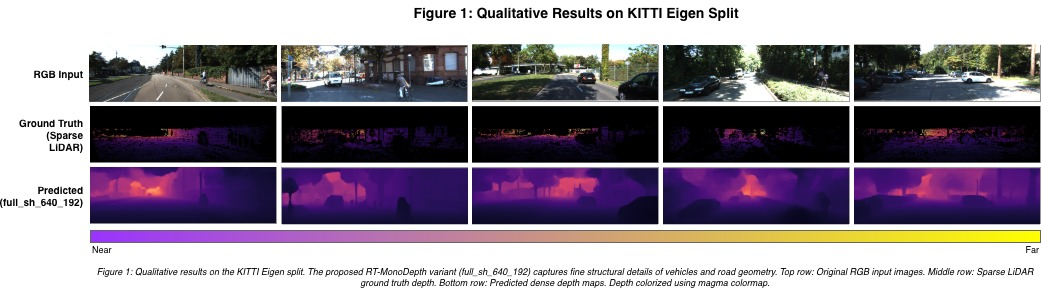
\includegraphics[width=0.85\linewidth]{figure3.png} 
    \caption{Qualitative results on the KITTI Eigen split. The proposed RT-MonoDepth variant (full\_sh\_640\_192) captures fine structural details of vehicles and road geometry. Top row: Original RGB input images. Middle row: Sparse LiDAR ground truth depth. Bottom row: Predicted dense depth maps.}
    \label{fig:qualitative_kitti}
\end{figure}

\begin{table}[H]
    \centering
    \caption{RT-MonoDepth Performance on KITTI Eigen Split (7,514 test images).}
    \label{tab:monodepth}
    \resizebox{\textwidth}{!}{%
    \begin{tabular}{lccccccc}
    \toprule
    \textbf{Model Variant} & $\delta < 1.25 \uparrow$ & $\delta < 1.25^2 \uparrow$ & $\delta < 1.25^3 \uparrow$ & AbsRel $\downarrow$ & SqRel $\downarrow$ & RMSE $\downarrow$ & RMSElog $\downarrow$ \\
    \midrule
    \textbf{full\_sh\_640\_192} & \textbf{96.09\%} & \textbf{99.1\%} & \textbf{99.8\%} & \textbf{0.0584} & \textbf{0.281} & \textbf{3.38m} & \textbf{0.089} \\
    full\_s\_640\_192 & 95.38\% & 98.9\% & 99.7\% & 0.0606 & 0.312 & 3.73m & 0.093 \\
    full\_m\_640\_192 & 95.38\% & 98.8\% & 99.7\% & 0.0615 & 0.298 & 3.64m & 0.092 \\
    full\_ms\_640\_192 & 95.59\% & 98.9\% & 99.7\% & 0.0625 & 0.305 & 3.65m & 0.094 \\
    s\_ms\_640\_192 & 93.69\% & 98.5\% & 99.5\% & 0.0749 & 0.398 & 4.29m & 0.108 \\
    s\_m\_640\_192 & 93.53\% & 98.4\% & 99.5\% & 0.0750 & 0.385 & 4.16m & 0.107 \\
    \bottomrule
    \end{tabular}%
    }
\end{table}

\subsubsection{Cross-Dataset Generalization}
To assess the system's robustness to domain shifts, we conducted a zero-shot transfer evaluation on the Cityscapes validation set (500 images) without prior fine-tuning. As shown in Table \ref{tab:cityscapes}, a significant performance gap exists between the source domain (KITTI: 96.09\%) and the target domain (Cityscapes: 38.25\%), highlighting the inherent challenges of domain adaptation. However, employing a weighted ensemble of all six variants combined with Test-Time Augmentation (TTA) yielded a substantial 14.4\% improvement in accuracy.

\begin{table}[H]
    \centering
    \caption{Cross-Dataset Evaluation (Cityscapes Validation Set)}
    \label{tab:cityscapes}
    \begin{tabular}{lcccc}
    \toprule
    \textbf{Approach} & $\delta < 1.25 \uparrow$ & AbsRel $\downarrow$ & RMSE $\downarrow$ & Improvement \\
    \midrule
    Single Model (full\_sh) & 38.25\% & 0.3736 & 18.16m & Baseline \\
    Weighted Ensemble + TTA & \textbf{52.65\%} & \textbf{0.2627} & \textbf{12.09m} & \textbf{+14.40\%} \\
    \bottomrule
    \end{tabular}
\end{table}

\subsection{Stage 2: Construction Safety Object Detection}
The second stage of our pipeline utilizes the YOLOv11n architecture \cite{jocher2024}, fine-tuned on the Construction Site Safety dataset \cite{roboflow2023} to detect 10 distinct classes, including Personal Protective Equipment (PPE) and heavy machinery.

\subsubsection{Dataset and Training Configuration}
The model was trained on 2,605 images with a $640 \times 640$ input resolution using the AdamW optimizer with an initial learning rate of 0.01 and momentum of 0.937. Representative samples are shown in Figure \ref{fig:dataset_samples}.

\begin{figure}[H]
    \centering
    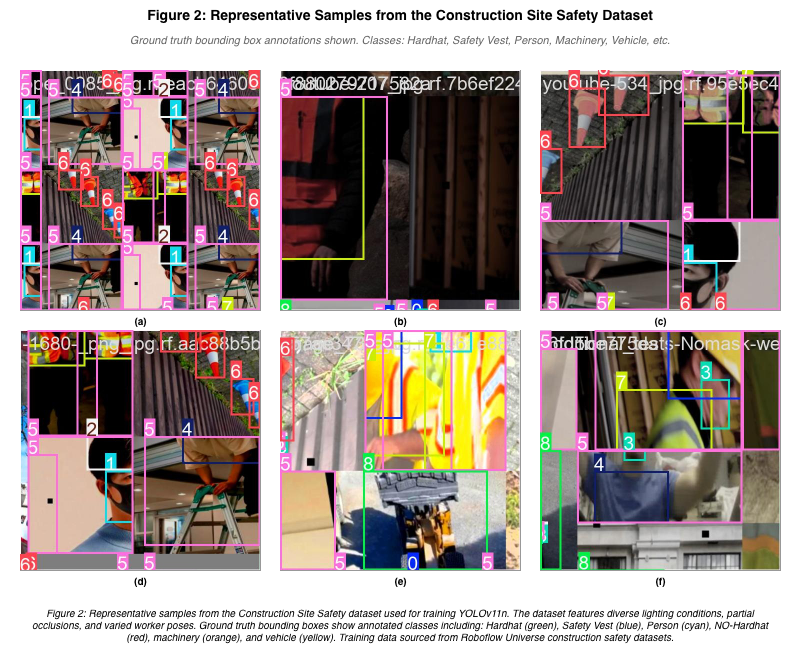
\includegraphics[width=0.50\linewidth]{figure4.png}
    \caption{Representative samples from the Construction Site Safety dataset used for training YOLOv11n. The dataset features diverse lighting conditions and partial occlusions.}
    \label{fig:dataset_samples}
\end{figure}

\subsubsection{Detection Performance Analysis}
The training progression is visualized in Figure \ref{fig:training_dynamics}. The model achieves stability in mAP@50 after approximately 150 epochs. At epoch 300, as shown in Table \ref{tab:yolo_milestones}, the model achieved a Precision of 95.18\% and an mAP@50 of 84.99\%. This high precision is particularly critical in safety monitoring to minimize false positives that could lead to alarm fatigue on construction sites.

Detections were further filtered using class-specific confidence thresholds (0.25 for "person" and 0.35 for other classes), with valid detections consistently exhibiting scores in the 0.35 to 0.89 range. Furthermore, a post-processing heuristic was successfully applied to reclassify large vehicles as machinery, enhancing contextual accuracy for construction site analysis.

\begin{figure}[H]
    \centering
    \includegraphics[width=\linewidth]{figure5.png}
    \caption{Training dynamics of YOLOv11n over 300 epochs. (a) Training Loss vs Epochs (b) mAP vs Epochs.}
    \label{fig:training_dynamics}
\end{figure}

\begin{table}[H]
    \centering
    \caption{YOLOv11n Performance Milestones}
    \label{tab:yolo_milestones}
    \begin{tabular}{lcccc}
    \toprule
    \textbf{Epoch} & \textbf{mAP@50} $\uparrow$ & \textbf{mAP@50-95} $\uparrow$ & \textbf{Precision} $\uparrow$ & \textbf{Recall} $\uparrow$ \\
    \midrule
    50 & 78.33\% & 45.34\% & 87.75\% & 72.02\% \\
    100 & 81.84\% & 54.29\% & 88.76\% & 77.22\% \\
    200 & 84.22\% & 59.47\% & 93.49\% & 77.85\% \\
    \textbf{300} & \textbf{84.99\%} & \textbf{60.06\%} & \textbf{95.18\%} & \textbf{77.87\%} \\
    \bottomrule
    \end{tabular}
\end{table}

\subsection{Stage 3: Deployment and Fusion}
To validate real-world utility, we optimized the inference pipeline for resource-constrained environments using ONNX Runtime and TensorRT.

\subsubsection{Synergistic Fusion Performance}
Initial performance testing was conducted on an Apple M1 Pro MacBook, where the system demonstrated a deployable inference speed of 22–25 FPS. To evaluate the feasibility of edge deployment on constrained hardware, the model was subsequently ported to a 2019 launched edge device (4GB).

Following specific optimization measures—including reducing input resolution, pruning the number of target classes, and converting the model to TensorRT—the system achieved a frame rate of 11 FPS at $320 \times 320$ resolution. Crucially, the synergistic fusion of the depth estimation and detection models validates the system's practical applicability for real-time deployment in resource-constrained safety monitoring scenarios.

\subsubsection{Geometric Calibration}
While the RT-MonoDepth module provides coherent depth maps, they are inherently scale-ambiguous. To resolve this for practical safety logging, an automatic geometric calibration function was employed. This method uses a detected "Person" as a reference object, acting as an anthropometric reference. Based on the pinhole camera model equation $Z=(f_y \cdot \text{ObjectHeight}_{\text{real}}) / \text{ObjectHeight}_{\text{pixels}}$, the system converts disparity outputs into meaningful metric measurements. This enables the subsequent 3D reconstruction pipeline to calculate accurate Euclidean distances between object pairs in real-time.

\subsection{Proximity Monitoring and Quantitative Logging}
The primary application of the framework—proactive safety monitoring—was validated through its depth logging feature. This functionality provides a quantitative, time-series analysis of the system's monitoring capabilities by continuously recording the spatial relationships between key objects.

\begin{figure}[H]
    \centering
    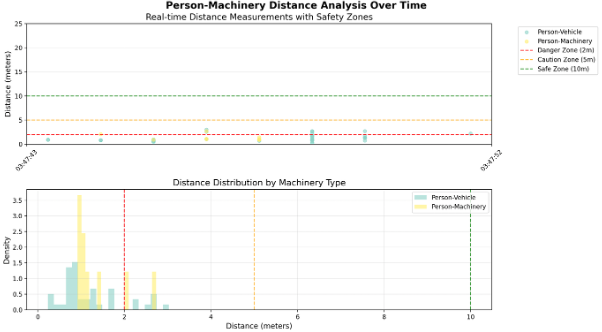
\includegraphics[width=\linewidth]{figure6.png}
    \caption{Person-Machinery Distance Analysis Over Time. A temporal plot visualizing the system's effectiveness in identifying potentially hazardous situations and flagging entries into "Caution" and "Danger" zones.}
    \label{fig:proximity_log}
\end{figure}

The system successfully tracked the evolving distances between detected personnel and active machinery throughout the test sequences. As illustrated in Figure \ref{fig:proximity_log}, the analysis revealed several instances where the separation distance fell below predefined safety thresholds, causing the system to correctly flag these events as entries into "Caution" and "Danger" zones. This result confirms that the framework can reliably detect proximity breaches in real time. The generated CSV logs serve as a persistent and actionable data source, suitable for post-incident analysis and integration with automated alert systems.

\subsection{LLM-Supervisor Evaluation with Llama~3.1 8B}
\label{sec:llm_results}
Following the protocol described in Section~\ref{sec:llm_supervisor_method}, we executed the full pipeline on a 2{,}998-frame construction-site recording (640$\times$360 at 25\,FPS, processed every third frame on an Apple~M1~Pro through MPS acceleration). The resulting depth log contained 1{,}031 rows with 137 valid object detections (96 \texttt{Person}, 30 \texttt{Vehicle}, 11 \texttt{Machinery}), and the distance log contained 19 pairwise rows. The thirty questions were then sent to a locally hosted Llama~3.1~8B Instruct model with temperature~$0$, an 8\,192-token context, and identical prompts.

The model achieved an aggregate accuracy of \textbf{10/30 = 33.3\%} across the benchmark, with a mean per-question latency of 3.95\,s and a total wall-clock time of 118.5\,s. The disaggregated per-category breakdown, presented in Table~\ref{tab:llm_supervisor}, exposes a strong capability gradient that is the central empirical finding of this evaluation:

\begin{itemize}
    \item \textbf{Row-level lookups (80\,\%).} When asked to retrieve a specific cell from a known row---``what is the depth of the first \texttt{Person} detection?'', ``what is the frame index of the first \texttt{Machinery} detection?''---the model is highly reliable, succeeding on 4 of 5 questions.
    \item \textbf{Class identification (67\,\%).} The model correctly identified the class with the highest mean confidence and the class with the largest mean depth, but mis-identified the class with the \emph{smallest} mean depth (predicted \texttt{Person}, ground truth \texttt{Machinery}; the values differ by only 0.20\,m). This boundary case suggests that small effect-size comparisons are unreliable.
    \item \textbf{Aggregate statistics (40\,\%).} Mean / max / min / median over many rows are computed correctly only intermittently. The model frequently anchors on a single visible row (e.g.\ reporting the \emph{first} \texttt{Person} depth, 2.05\,m, in place of the true mean, 2.73\,m).
    \item \textbf{Counts (20\,\%).} The model nearly always over- or under-counted detections by a small but non-trivial margin (e.g.\ predicting 67 instead of 96 \texttt{Person} rows, 17 instead of 11 \texttt{Machinery} rows), consistent with known limitations of transformer LMs on integer enumeration over long contexts.
    \item \textbf{Threshold-based proximity reasoning (0\,\%).} Most strikingly, the model failed every single question that required filtering rows by a safety threshold (Danger / Caution / Safe zones) or computing the minimum distance restricted to a particular class pair. Several failures were not minor numeric errors but extreme hallucinations in which the model returned a \emph{frame index} (e.g.\ 2{,}833 or 1{,}183) in place of a row count.
    \item \textbf{Supervisory safety decisions (33\,\%).} On the three yes/no decision questions, the model contradicted the ground truth on the first ``did any pairwise distance involving a Person fall below 1\,m?'' (predicted \texttt{no}, truth \texttt{yes}), but correctly issued a \texttt{yes} workflow-review recommendation when the question was reframed with the rule made explicit.
\end{itemize}

\begin{table}[H]
    \centering
    \caption{Per-category accuracy of the locally hosted Llama~3.1 8B supervisor on the thirty automatically graded questions. Ground truth is computed deterministically from the CSV logs produced by the perception pipeline.}
    \label{tab:llm_supervisor}
    \begin{tabular}{lccc}
    \toprule
    \textbf{Category} & \textbf{Correct} & \textbf{Total} & \textbf{Accuracy} \\
    \midrule
    Row-level lookup           & 4 & 5 & 80.0\% \\
    Class identification       & 2 & 3 & 66.7\% \\
    Aggregate (depth + conf.)  & 2 & 5 & 40.0\% \\
    Safety decision (yes/no)   & 1 & 3 & 33.3\% \\
    Counts (long-context)      & 1 & 5 & 20.0\% \\
    Proximity-zone reasoning   & 0 & 6 & 0.0\% \\
    Distinct-frame reasoning   & 0 & 3 & 0.0\% \\
    \midrule
    \textbf{Overall}           & \textbf{10} & \textbf{30} & \textbf{33.3\%} \\
    \bottomrule
    \end{tabular}
\end{table}

This monotonically degrading accuracy curve---from 80\,\% on lookups, through 40\,\% on aggregates, to 0\,\% on threshold filtering---provides direct empirical evidence that an 8B-parameter local LLM can be safely used to \emph{paraphrase} and \emph{retrieve} entries from the perception logs but must \emph{not} be trusted to recompute safety statistics on its own. The deterministic CSV pipeline, not the LLM, must remain the system of record. We discuss the deployment implications of this finding in Section~\ref{sec:discussion_llm}.

\section{Discussion and Limitations}
The results presented in this study validate the core hypothesis that a synergistic fusion of real-time object detection and monocular depth estimation can create a cost-effective and powerful safety monitoring tool. Our framework successfully demonstrates the ability to move beyond generic depth maps and provide object-specific, actionable spatial data from a single 2D camera.

The system's performance, achieving 96.09\% depth accuracy and 84.99\% detection mAP, highlights the robustness of the chosen architecture. Deployment tests confirmed the system's efficiency on edge devices. While the edge device represents older hardware, the achievement of 11 FPS (and 22–25 FPS on Apple Silicon) confirms suitability for real-time applications where immediate feedback is paramount for accident prevention \cite{feng2024}. This capability is a direct result of the multi-threaded, parallel processing architecture that executes the YOLOv11 and RT-MonoDepth models concurrently.

However, the cross-dataset evaluation reveals a 43\% performance drop when transferring from KITTI to Cityscapes, indicating a need for unsupervised domain adaptation. Additionally, while the $320 \times 320$ resolution enables real-time performance on the edge device, it limits the detection of small, distant safety violations (e.g., a missing helmet at $>20$ meters).

Furthermore, the auto-calibration mechanism is dependent on the presence of a "person" in the camera's field of view and assumes a static average height of 1.7 meters. The system's reliability could be compromised in scenarios where no personnel are visible, or when personnel height deviates significantly from the average. Future iterations could explore more robust calibration techniques, such as using multiple object classes for reference or incorporating self-supervised scale recovery methods that do not rely on specific object detection \cite{shen2023}.

\subsection{Implications of the LLM-Supervisor Evaluation}
\label{sec:discussion_llm}
The thirty-question Llama~3.1 8B benchmark in Section~\ref{sec:llm_results} also has direct design consequences for the broader ``LLM-on-top-of-CV'' deployment pattern. Three implications stand out.

First, \emph{the deterministic perception layer must remain authoritative for any safety-critical aggregate}. Counts of close-call events, time spent in the Danger zone, or class-restricted minimum distances should be computed by the pipeline (or by SQL/pandas) and \emph{rendered} into the prompt as pre-computed numbers, rather than asked of the LLM as a free-form question. Our 0\,\% accuracy on threshold-based proximity reasoning shows that this is not a hyperparameter problem to be tuned away with prompt engineering---it is a fundamental capability gap of small open-weight models on tabular data.

Second, \emph{LLM supervision is most valuable as a retrieval and explanation layer}. The 80\,\% accuracy on row-level lookups indicates that a small local model is well suited to answering ``what was the depth of the worker the system flagged at frame 1{,}492?''---i.e.\ explaining a single event the deterministic pipeline has already surfaced---rather than re-deriving the event itself. This suggests a hybrid architecture in which the pipeline's incident detector emits a structured event, and the LLM's only job is to verbalize the event in human-readable language for the supervisor's dashboard.

Third, \emph{automated, ground-truth-grounded benchmarks are themselves a contribution}. By treating the CSV logs as the source of truth and the LLM as a system under test, our protocol turns a vague claim (``our LLM is reasonable for safety summaries'') into a falsifiable, reproducible statistic (33.3\,\% overall, 0\,\% on threshold reasoning). We argue that papers proposing LLM-based safety dashboards should be expected to report comparable numbers, and we release \texttt{llm\_supervisor\_eval.py} so that other authors can reuse the protocol against larger models, fine-tuned variants, or tool-augmented agents (e.g.\ models that can issue pandas queries against the log) and quantitatively measure the resulting improvement.

\section{Conclusion}
This work presented a real-time safety perception system achieving 96.09\% depth accuracy and 84.99\% detection mAP. By optimizing the pipeline with TensorRT and FP16 precision, we demonstrated the feasibility of running complex, multi-stage AI on embedded hardware, paving the way for automated, low-cost safety monitoring on active construction sites.

The key contribution of this work lies in its synergistic approach, fusing state-of-the-art perception models like YOLOv11 \cite{jocher2024} for intelligent recognition into a unified, deployable tool. The implementation of an automatic geometric calibration function proved effective for resolving scale ambiguity, enabling accurate 3D reconstruction and Euclidean distance calculations. Empirical validation through quantitative logging confirmed the system's ability to reliably detect and flag proximity breaches against predefined safety zones, presenting a viable path toward reducing the high rate of fatalities in the construction industry.

Beyond perception accuracy, this paper also introduces an automatically graded LLM-supervisor benchmark in which thirty ground-truth-grounded questions are answered by a locally hosted Llama~3.1 8B model. The resulting capability profile (80\,\% on lookups, 0\,\% on threshold-based proximity reasoning, 33.3\,\% overall) provides the first quantitative answer---specific to construction safety---to the question of \emph{which natural-language queries an on-device LLM can be trusted to answer from a deterministic perception pipeline}, and motivates a hybrid architecture in which the LLM verbalizes events flagged by the pipeline rather than recomputing them. The full evaluation harness is released alongside the perception code as \texttt{process\_video\_headless.py} and \texttt{llm\_supervisor\_eval.py} to enable apples-to-apples comparisons against future LLMs.

% IEEE Style Bibliography
\begin{thebibliography}{99}

\bibitem{feng2024}
C. Feng et al., ``Real-time monocular depth estimation on embedded systems,'' in \textit{Proc. IEEE Int. Conf. Multimedia Expo (ICME)}, 2024.

\bibitem{geiger2012}
A. Geiger, P. Lenz, and R. Urtasun, ``Are we ready for autonomous driving? The KITTI vision benchmark suite,'' in \textit{Proc. IEEE Conf. Comput. Vis. Pattern Recognit. (CVPR)}, 2012, pp.~3354--3361.

\bibitem{he2024}
L. He, Y. Zhou, L. Liu, and J. Ma, ``Research and application of YOLOv11-based object segmentation in intelligent recognition at construction sites,'' \textit{Buildings}, vol.~14, no.~12, p.~3777, 2024.

\bibitem{jocher2024}
G. Jocher et al., \textit{Ultralytics YOLO11}. Ultralytics, 2024. [Online]. Available: \url{https://github.com/ultralytics/ultralytics}

\bibitem{masoumian2022}
A. Masoumian, H. A. Rashwan, J. Cristiano, M. S. Asif, and D. Puig, ``Monocular depth estimation using deep learning: A review,'' \textit{Sensors}, vol.~22, no.~14, p.~5353, 2022.

\bibitem{pan2021}
Y. Pan and L. Zhang, ``Roles of artificial intelligence in construction engineering and management: A critical review and future trends,'' \textit{Autom. Constr.}, vol.~122, p.~103517, 2021.

\bibitem{roboflow2023}
Roboflow Universe Projects, ``Construction site safety dataset,'' Roboflow, 2023. [Online]. Available: \url{https://universe.roboflow.com/roboflow-universe-projects/construction-site-safety}

\bibitem{shen2023}
J. Shen, W. Yan, S. Qin, and X. Zheng, ``A self-supervised monocular depth estimation model with scale recovery and transfer learning for construction scene analysis,'' \textit{Comput.-Aided Civ. Infrastruct. Eng.}, vol.~38, no.~9, pp.~1142--1161, 2023.

\bibitem{yu2021}
J. Yu and H. Choi, ``YOLO MDE: Object detection with monocular depth estimation,'' \textit{Electronics}, vol.~11, no.~1, p.~76, 2021.

\bibitem{zhang2025}
Z. Zhang, Y. Zhang, Y. Li, and L. Wu, ``Review of monocular depth estimation methods,'' \textit{J. Electron. Imag.}, vol.~34, no.~2, p.~020901, 2025.

\bibitem{dubey2024llama}
A. Dubey, A. Jauhri, A. Pandey et al., ``The Llama 3 herd of models,'' \textit{arXiv preprint} arXiv:2407.21783, 2024.

\bibitem{ollama2024}
Ollama, ``Ollama: Get up and running with large language models locally,'' 2024. [Online]. Available: \url{https://ollama.com}

\bibitem{adil2025}
M. Adil, G. Lee, V. A. Gonz\'{a}lez, and Q. Mei, ``Using vision language models for safety hazard identification in construction,'' \textit{arXiv preprint} arXiv:2504.09083, 2025.

\bibitem{badhan2025}
S. J. Badhan and R. Samsami, ``Artificial intelligence (AI) in construction safety: A systematic literature review,'' \textit{Buildings}, vol.~15, no.~22, p.~4084, 2025.

\bibitem{cai2025}
R. Cai, J. Li, Y. Tan, J. Tang, and X. Chen, ``Convolutional neural networks for construction safety: A technical review of computer vision applications,'' \textit{Appl. Soft Comput.}, vol.~180, p.~113374, 2025.

\bibitem{cheng2025}
Z. Cheng, T. Liu, T. Lei, X. Hua, Y. Zhang, and C. Tang, ``RTS-Mono: A real-time self-supervised monocular depth estimation method for real-world deployment,'' \textit{arXiv preprint} arXiv:2511.14107, 2025.

\bibitem{ge2025}
T. Ge, B. Ning, and Y. Xie, ``YOLO-AFR: An improved YOLOv12-based model for accurate and real-time dangerous driving behavior detection,'' \textit{Appl. Sci.}, vol.~15, no.~11, p.~6090, 2025.

\bibitem{huang2025}
Z. Huang, M. A. H. Ali, Y. Nukman, H. L. Xu, S. Zhang, H. Chen, and M. Alkhedher, ``A systematic review of monocular depth estimation for autonomous driving: Methods and dataset benchmarking,'' \textit{Results Eng.}, vol.~26, p.~105359, 2025.

\bibitem{lee2024}
J. Lee, S. Ahn, D. Kim, and D. Kim, ``Performance comparison of retrieval-augmented generation and fine-tuned large language models for construction safety management knowledge retrieval,'' \textit{Autom. Constr.}, vol.~168, p.~105846, 2024.

\bibitem{ma2026}
L. Ma, Y. Li, B. Jiang, Z. Zhong, H. Ding, and L. Zhu, ``AsyncMDE: Real-time monocular depth estimation via asynchronous spatial memory,'' \textit{arXiv preprint} arXiv:2603.10438, 2026.

\bibitem{samsami2024}
R. Samsami, ``Optimizing the utilization of generative artificial intelligence (AI) in the AEC industry: ChatGPT prompt engineering and design,'' \textit{CivilEng}, vol.~5, no.~4, pp.~971--1010, 2024.

\bibitem{vasquez2025}
E. Vasquez, M. Hale, and S. Chen, ``Computer vision applications for real-time safety monitoring on construction sites,'' ResearchGate, 2025.

\bibitem{wang2025}
C. Wang et al., ``Automating construction safety inspections using a multi-modal vision-language RAG framework,'' \textit{arXiv preprint} arXiv:2510.04145, 2025.

\bibitem{zhang2024helmets}
L. Zhang, Z. Sun, H. Tao, Y. Liu, X. Guo, and J. Chen, ``Research on mine-personnel helmet detection based on multi-strategy-improved YOLOv11,'' \textit{Sensors}, vol.~25, no.~1, p.~170, 2024.

\end{thebibliography}

\end{document}
